\documentclass[a4paper]{report}

% Paquetes
% CUIDADO: alterar el orden puede generar errores inesperados
% ============================================================================ %
\usepackage[spanish]{babel} % Paquete para utilizar el idioma español
\usepackage[utf8]{inputenc} % Codificación de caracteres UTF-8
\usepackage{setspace} % Para ajustar el espaciado entre líneas
\usepackage{titlesec} % Para personalizar los encabezados de capítulos y secciones
\usepackage{lipsum} % Para generar texto ficticio, puedes eliminar esta línea
\usepackage{enumitem} % Para enumerar items
\usepackage[hidelinks]{hyperref} % Para generar los enlaces a las secciones correspondientes
\usepackage{geometry} % Permite ajustar y modificar los márgenes y dimensiones de la página en LaTeX.
\usepackage{graphicx} % Proporciona comandos para incluir y manipular imágenes en LaTeX.
\usepackage{fancyhdr} % Permite personalizar el encabezado y pie de página en LaTeX.
\usepackage{microtype} % Mejora la apariencia del texto ajustando el espaciado entre caracteres y palabras.
\usepackage{chngcntr} % Permite cambiar el formato y numeración de los contadores en LaTeX.
\usepackage{tocbibind} % Controla la inclusión de elementos como la tabla de contenido, lista de figuras y lista de tablas en el índice general.
\usepackage{array} % Amplía las capacidades de las tablas en LaTeX, permitiendo personalizar el formato y comportamiento de las celdas.
\usepackage{cellspace} % Proporciona espacios adicionales en las celdas de las tablas para mejorar su apariencia.
\usepackage[acronym]{glossaries} % Facilita la creación y gestión de glosarios y listas de acrónimos en LaTeX.
\usepackage{float} % Proporciona mejoras en el posicionamiento de objetos flotantes, como figuras y tablas, en LaTeX.
\usepackage{fontspec} % Permite la selección y configuración de fuentes tipográficas en LaTeX.
\usepackage{amsmath} % Mejora la calidad tipográfica de las fórmulas matemáticas y proporciona comandos y entornos adicionales.
\usepackage{xcolor} % Amplía las capacidades de color en LaTeX, permitiendo el uso de colores personalizados.
\usepackage{listings} % Facilita la inclusión y formateo de código fuente en documentos LaTeX.
% ============================================================================ %

% Otras configuraciones del preámbulo
\hypersetup{
  pdftitle={Sistema de Transmisión AM con Codificación DTMF},
  pdfauthor={Boeri, Benjamin; Campero, Leandro; Villafañe, Cristian},
  pdfsubject={Informe de Trabajo Integrador - Procesamiento Digital de Señales 2022},
  pdfkeywords={PDS, Informe, Boeri, Campero, Villafañe, 2022},
  pdfproducer={LaTeX},
  pdfcreator={pdfLaTeX}
}

% Header y footer
\pagestyle{fancy}
\fancyhf{}
\lhead{Procesamiento Digital de Señales}
\rhead{Trabajo Integrador}
\lfoot{\nouppercase{\leftmark}}
\rfoot{\thepage}

\fancypagestyle{plain}{
  \fancyhf{}
  \lhead{Procesamiento Digital de Señales}
  \rhead{Trabajo Integrador}
  \lfoot{\nouppercase{\leftmark}}
  \rfoot{\thepage}
}

\fancyhfoffset[R]{0pt} % Ajusta el ancho del encabezado
\fancyhfoffset[L]{0pt} % Ajusta el ancho del pie de página

\newgeometry{
  top=1.25in,
  bottom=1in,
  outer=0.75in,
  inner=0.75in,
}

% Configuración de página
\setlength{\parindent}{0pt} % Deshabilitar sangría al inicio de párrafos
\setlength{\parskip}{1em} % Establecer espaciado entre párrafos

% Personalizaciones
\titleformat{\chapter}[display]
{\normalfont\huge\bfseries}{\chaptertitlename\ \thechapter}{20pt}{\Huge}
\titlespacing*{\chapter}{0pt}{0pt}{40pt} % Ajustar espaciado antes y después de los encabezados de capítulo

% Tamaño de fuente e interlineado
\renewcommand{\normalsize}{\fontsize{12}{14}\selectfont}

\counterwithout{table}{section} % Desvincular el contador de las tablas de las secciones
\counterwithout{figure}{section} % Desvincular el contador de las figuras de las secciones
\counterwithin{table}{chapter} % Vincular el contador de las tablas al contador de los capítulos
\counterwithin{figure}{chapter} % Vincular el contador de las figuras al contador de los capítulos
\setlength{\tabcolsep}{10pt} % Espaciado horizontal
\setlength{\extrarowheight}{5pt} % Espaciado vertical

\newcommand{\titulo}{Sistema de Transmisión AM con Codificación DTMF}
\newcommand{\subtitulo}{Informe de Trabajo Integrador}
\newcommand{\materia}{Procesamiento Digital de Señales}
\newcommand{\unidadacademica}{Facultad de Ciencias Exactas y Tecnología}
\newcommand{\universidad}{Universidad Nacional de Tucumán}
\newcommand{\autores}{
  Boeri, Benjamin \\
  Campero, Leandro \\
  Villafañe, Cristian
}
\newcommand{\fecha}{\today}

% Comienza el documento
\begin{document}

% Página de título
\begin{titlepage}
  \centering


  \begin{spacing}{2}
    \textbf{\Huge \titulo}
  \end{spacing}

  \Large \subtitulo

  \vspace{1cm}

  
\includegraphics[width=6cm]{images/logo_unt.png}

  \textbf{\large \materia}

  \textbf{\large \unidadacademica}

  \textbf{\large \universidad}

  \vspace{0.5cm}

  \textbf{\Large Autores:}

  \autores

  \vfill

  \Large \fecha

\end{titlepage}

% Resumen
\begin{abstract}
  El procesamiento digital de señales se refiere a la manipulación, análisis y transformación de señales utilizando algoritmos y técnicas computacionales. En este proyecto, el procesamiento digital de señales se aplica para generar y decodificar los tonos DTMF, así como para simular la transmisión y detección de los dígitos enviados.

  Este proyecto presenta la implementación de un sistema de Modulación en Amplitud (AM) y Codificación DTMF utilizando MATLAB/SIMULINK. Se busca transmitir dígitos numéricos codificados en DTMF a través de un enlace cableado simulado. El sistema involucra la generación de tonos DTMF, el diseño de filtros digitales pasa bandas para el decodificador, la configuración de la frecuencia de portadora RF y la modelización del canal de transmisión como un filtro analógico pasa banda.

  Un filtro digital es un componente esencial en el procesamiento digital de señales que permite modificar las características de una señal. En este proyecto, se utilizan filtros digitales pasa bandas implementados mediante la técnica del filtro Butterworth. Estos filtros permiten seleccionar y aislar las frecuencias específicas asociadas a los tonos DTMF.

  La implementación de los filtros digitales se logra mediante la transformación de los coeficientes del filtro en una representación numérica que se aplica a la señal de entrada. Esto puede lograrse utilizando algoritmos y técnicas de programación, así como también herramientas como MATLAB y SIMULINK.

  El resultado de este proyecto demuestra la viabilidad y efectividad de la implementación del sistema propuesto. El procesamiento digital de señales y el uso de filtros digitales son fundamentales en diversas aplicaciones, incluyendo las comunicaciones y el procesamiento de señales de audio.

  En resumen, este proyecto combina el procesamiento digital de señales, la modulación AM, el diseño de filtros digitales y la codificación DTMF para lograr la transmisión y detección de dígitos numéricos. La implementación exitosa de este sistema contribuye al avance y comprensión de las técnicas de procesamiento y transmisión de señales en el ámbito de las comunicaciones.
\end{abstract}


% Índice
\tableofcontents

% Introduccion
% Capítulo 1
\chapter{Introducción}
\section{Problema propuesto}
La modulación en amplitud o \gls{am},
permite la transmisión de una señal de
baja frecuencia superpuesta a una onda
de alta frecuencia. Este sistema de
modulación permite enviar mensajes en
la forma de envolventes de la onda
portadora, ya sea por un canal de aire o
físico utilizando un enlace cableado.\\
El sistema de codificación \gls{dtfm}, utiliza una
combinación de tonos de frecuencia
audibles pera representar el conjunto de
números del 0 al 9 disponible en el
teclado telefónico, con lo cual es posible
enviar una codificación numérica por la
línea telefónica.\\
El modelo de trabajo está representado
en la Figura \ref{fig:intro_diagrama_bloques}, correspondientes al
Modulador y Demodulador \gls{am}, el canal
de cable telefónico, y las etapas de
codificación y decodificación \gls{dtfm}.

\begin{figure}[ht]
  \centering
  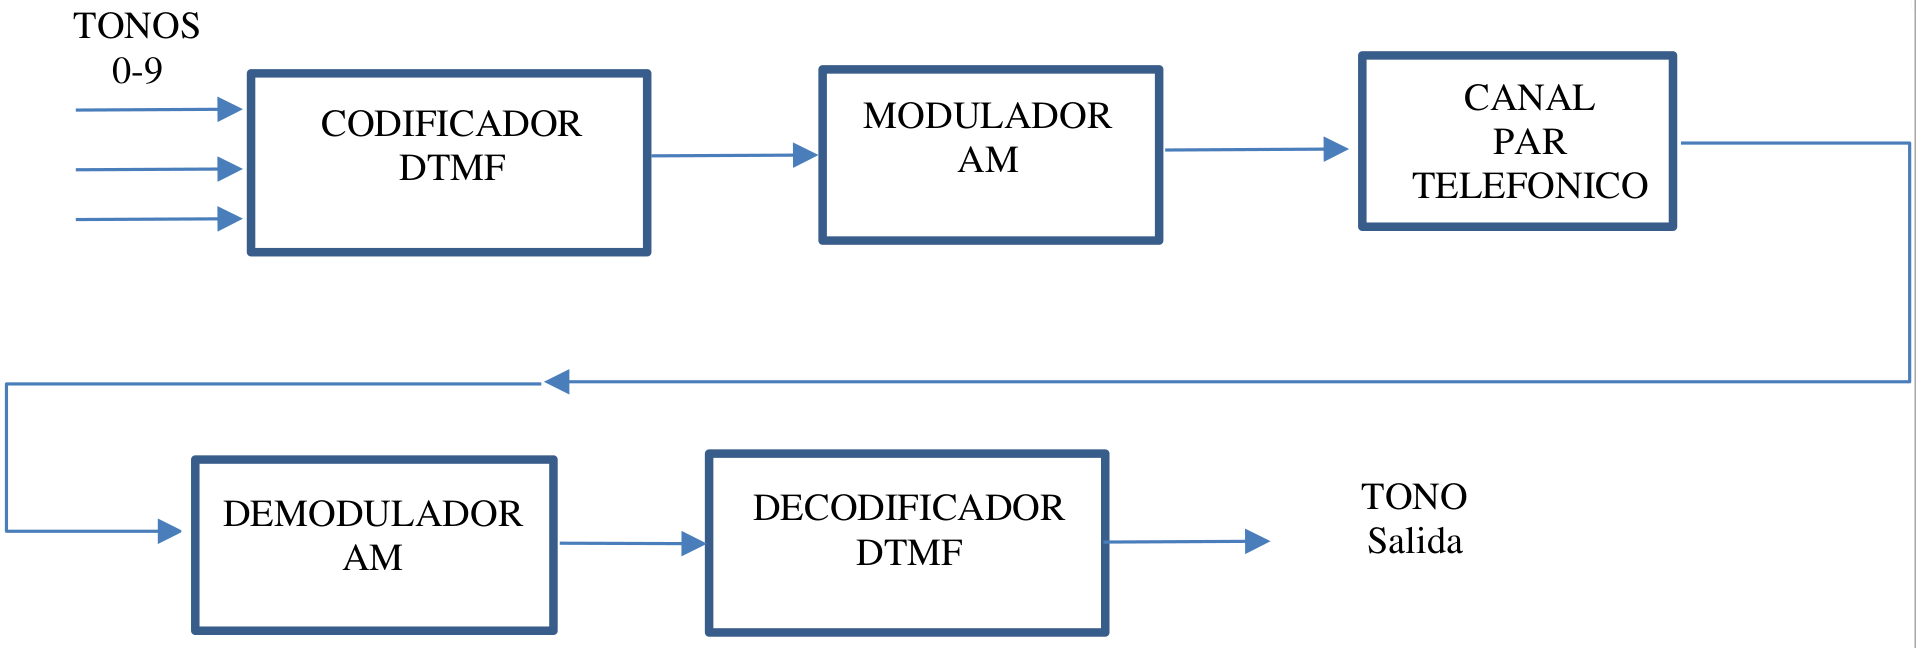
\includegraphics[width=\linewidth]{images/intro_diagrama_general.png}
  \caption{Diagrama de bloques general}
  \label{fig:intro_diagrama_bloques}
\end{figure}

\section{Objetivo}
El objetivo principal de este proyecto
integrador es la implementación del
sistema mostrado en la Figura \ref{fig:intro_diagrama_bloques},
utilizando MATLAB, SIMULINK, o la
combinación de ambos recursos de
modelado computacional, para el
envío de números (0-9) codificados
en \gls{dtfm} bajo modulación \gls{am}, y la
detección del número enviado a la
salida (uno número cada por vez).\\
A modo de referencia, el Cuadro \ref{tab:combinacion_tonos},
muestra la combinación de tonos
audibles asociados al conjunto
numérico, y en el enlace indicado
se encuentra la información ampliada
sobre la codificación \gls{dtfm}.

\begin{table}[htbp]
  \centering
  \begin{tabular}{|Sc|Sc|Sc|Sc|}
    \hline
    \textbf{Frecuencia Baja} & \textbf{Frecuencia Alta} & \textbf{Digito} & \textbf{Frecuencia Final} \\
    \hline
    697                      & 1209                     & 1               & 1906                      \\ \hline
    697                      & 1336                     & 2               & 2033                      \\ \hline
    697                      & 1477                     & 3               & 2174                      \\ \hline
    770                      & 1209                     & 4               & 1979                      \\ \hline
    770                      & 1336                     & 5               & 2106                      \\ \hline
    770                      & 1477                     & 6               & 2247                      \\ \hline
    852                      & 1209                     & 7               & 2061                      \\ \hline
    852                      & 1336                     & 8               & 2188                      \\ \hline
    852                      & 1477                     & 9               & 2329                      \\ \hline
    941                      & 1336                     & 0               & 2277                      \\
    \hline
  \end{tabular}
  \caption{Combinación de tonos audibles (medido en [Hz])}
  \label{tab:combinacion_tonos}
\end{table}

\section{Enunciado}
\begin{enumerate}[label=\alph*)]
  \item A nivel simulación se deberán sintetizar
        los tonos asociados a cada digito
        numérico seleccionando la frecuencia
        de muestreo $F_S$ apropiada (Teorema de Nyquist-Shannon).
  \item El demodulador \gls{dtfm} deberá ser
        implementado mediante filtros
        digitales pasa bandas, con un
        orden y respuestas apropiadas. El
        modo de indicar cuál fue el digito
        enviado queda a criterio del grupo
        de trabajo.
  \item Para el modelo de trasmisión AM
        (enlace cableado) se deberán
        establecer y sintetizar la frecuencia
        de portadora $RF$ el índice de
        modulación apropiados
        (recordando que la $F_S$ es única en
        todo el sistema).
  \item El canal de transmisión se
        corresponde al de un filtro
        analógico (transformado a digital)
        pasa banda con un rango de 300 Hz
        a 3400 Hz, respuesta plana y orden
        apropiado. Se considera el rango
        útil asignado a la frecuencia
        telefónica, aunque el cable
        telefónico de cobre tipo AWG-24,
        por ejemplo, supera este ancho de
        banda a 1Mz en distancias
        inferiores a 200 Mts.
\end{enumerate}

\section{Lineamientos Generales}
\begin{enumerate}[label=\alph*)]
  \item El grupo de trabajo deberá cumplir con las especificaciones del proyecto,
        utilizando criterios de diseños justificados para cada bloque del sistema.
  \item Se deberán indicar el paso a paso para el diseño de los filtros digitales utilizados
        en las diferentes etapas.
  \item El criterio de selección para el filtro analógico representativo del canal ( Bessel,
        Butterworth, etc.), y el método de transformación analógico a discreto escogido,
        brindando una gráfica comparativa de la respuesta en frecuencia resultantes en ambos
        planos (Laplace y Z).
  \item Se pide 3 aplicaciones posibles del sistema desarrollado en aplicaciones de tele
        comando (por ejemplo, aplicación de sistema de riego por comando telefónico de
        3 zonas), y como se imprentaría en la práctica (no el desarrollo, solo la propuesta).
  \item Problema de análisis: para el caso de que ocurran fallos en el canal de comunicación
        (por ejemplo, una atenuación en determinadas frecuencias), analizar la robustez del
        código detector para al menos 3 zonas atenuadas de frecuencias diferentes. Utilizar
        el código adjunto en Matlab para el diseño del canal con fallas. Justificar los
        resultados.
  \item Escribir el informe, Incluir conclusiones, observaciones y sugerencias sobre los
        resultados obtenidos
\end{enumerate}

% Planteamiento
\chapter{Planteamiento}
\section{Sistema}
Lo que se busca es simular un sistema \gls{dtfm} cuya señal se transmite a través de un canal telefónico con modulación \gls{am}. Tal simulación debe comprender cada uno de los bloques intervinientes en el sistema, como se muestra en la Figura \ref{fig:diagrama_bloques_objetivo}. Antes de diseñar y planificar la simulación hay que tener en cuenta las frecuencias intervinientes, particularmente hablando de la \gls{fp} (que determina la frecuencia de la señal a ser modulada en la transmisión) y la \gls{fs} (que determina la cantidad de muestras por segundo para la simulación).

Ya que esta simulación trata de la transmisión en \gls{am} a través de un canal telefónico, podemos tomar una \gls{fs} utilizada universalmente en sistemas de audio, y esta equivale a 44 [kHz], y podemos ver que claramente cumple con el Teorema de Nyquist-Shannon ya que es mayor al doble de la señal de mayor frecuencia (1477 [Hz], componente alta de los digitos 3, 6 y 9). Para la \gls{fp} tomamos 15 [kHz] ya que es 10 veces mayor a la señal antes mencionada y es menor a la mitad de \gls{fs} (para poder seguir cumpliendo con el teorema).

A continuación enumeramos el tratamiento de la señal en cada bloque del sistema:

\begin{enumerate}
  \item Codificador DTMF: Se suman las señales sinusoidales correspondientes a las frecuencias que componen cada digito
  \item Modulador AM: Se modula la señal portadora con la señal codificada
  \item Cable Telefónico: La señal modulada pasa por un filtro pasa-banda para simular el canal de voz [300-3300][Hz]
  \item Demodulador AM: Se bate la señal recibida con la misma portadora para obtener la moduladora
  \item Decodificador DTMF: La señal pasa por un banco de filtros pasa-banda para determinar qué señales de la matriz fueron enviadas
\end{enumerate}

\begin{figure}[H]
  \centering
  
\includegraphics[width=\linewidth]{images/planteamiento/bloques.png}
  \caption{Diagrama de bloques a simular}
  \label{fig:diagrama_bloques_objetivo}
\end{figure}

\section{Decodificación}
Para decodificar la señal del tono se tiene que implementar un banco de filtros en base a la matriz de señales del sistema \gls{dtfm}. Esto es, las filas se corresponden con las frecuencias bajas y las columnas con las frecuencias altas. La sumatoria de las señales se corresponde con la codificación del tono propuesto; esta señal llega a la matriz para devolver el tono correspondiente. El bloque decodificador se compone de filtros pasa-banda para cada frecuencia y el bloque detector como muestra la Figura \ref{fig:diagrama_bloques_decod}. La razón de usar un filtro para cada frecuencia baja y alta, en lugar de un filtro por cada frecuencia resultante, se debe a que de esta forma usamos 7 filtros en lugar de 9 (uno por cada tono); además, estas frecuencias (altas y bajas) están más separadas en el espectro que las frecuencias resultantes, lo cual es provechoso a la hora de diseñar un filtro.

La matriz será un bloque lógico que devolverá el digito correspondiente en base a las señales que hayan logrado activarse luego pasar por el banco de filtros.

\begin{figure}[H]
  \centering
  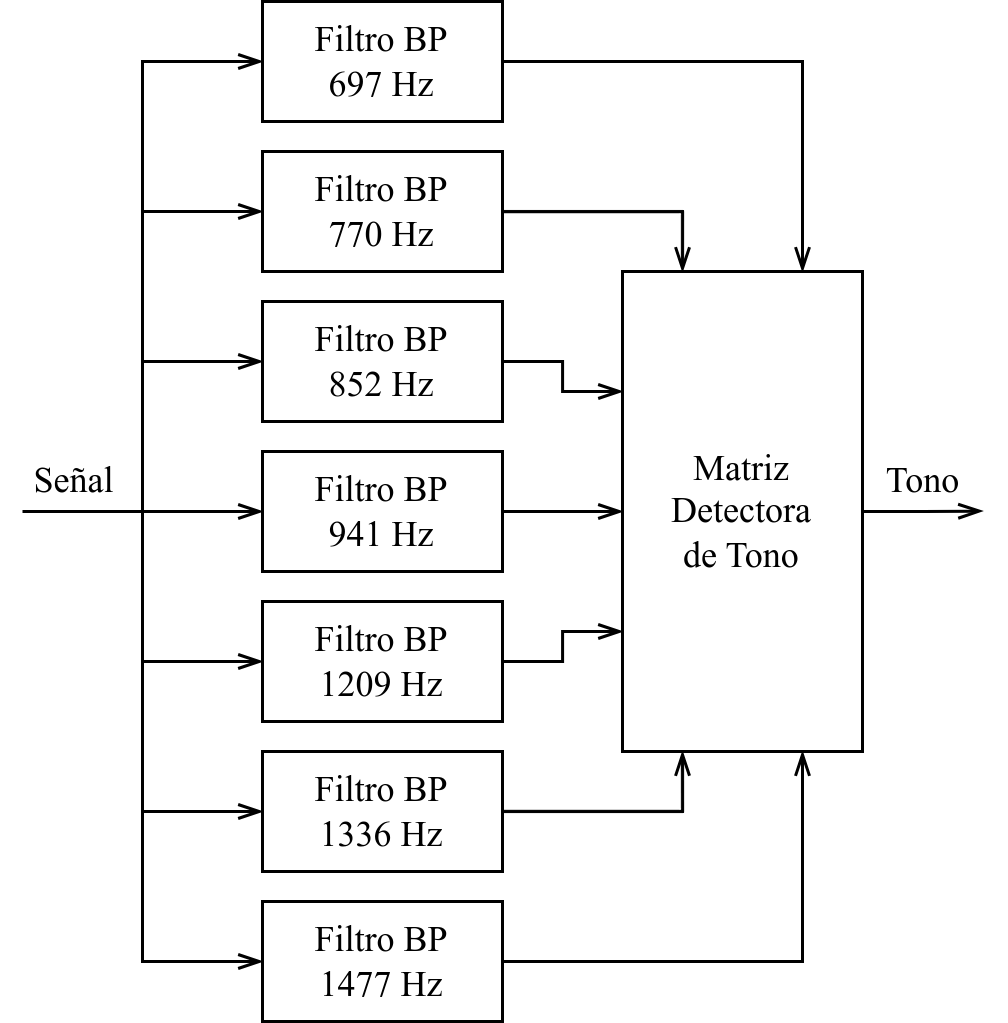
\includegraphics[width=300pt]{images/planteamiento/decodificador.png}
  \caption{Composición del bloque decodificador}
  \label{fig:diagrama_bloques_decod}
\end{figure}

\section{Simulación}
La simulación de este sistema, que es el objetivo de este proyecto, se logrará a través del uso de distintas herramientas dentro del software MATLAB. Entre estas herramientas se encuentra simulink que sirve para realizar el estudio en el tiempo y frecuencia de las señales a través de cada bloque del sistema.

Cada señal de entrada al sistema será simulada a través de generadores de sinusoidales, mientras que los filtros serán bloques que actuen en base a polinomios obtenidos por librerías provistas por MATLAB. El resto de las herramientas serán provistas por simulink (sumadores, multiplicadores, analizadores de espectro, etc.)

La razón de usar una herramienta para el diseño de los filtros es que estos se presumen de alto orden, lo cual es engorroso de calcular de manera analítica. Sin embargo, con el objetivo de comprender cómo es el diseño de filtros digitales, se explicará en el siguiente capítulo cómo es el proceso de diseño y análisis correspondiente.

% Filtros Digitales
\chapter{Filtros Digitales}
\section{Especificaciones}

\section{Diseño}

\section{Conversión de Analógico a Digital}

\section{Análisis}

\section{Conclusiones}

% Desarrollo
\chapter{Desarrollo}
Recordemos de la Figura \ref{fig:diagrama_bloques_objetivo} que nuestro sistema está compuesto por 5 bloques. En este capítulo vamos descomponer y analizar cada bloque para su posterior implementación en la simulación.

\section{Análisis}
\subsection*{Codificador y Modulador}
Estos bloques son en realidad bastante simples. Consta de la sumatoria de dos señales sinusoidales. Para la simulación serían dos generadores establecidos en la combinación de frecuencias que corresponden a un determinado digito. Para crear la codificación, basta con ingresar ambas señales a un sumador. Esto luego debe sumarse a una señal constante de 1, con el fin de poder hacer el producto de la señal resultante con la señal portadora. El resultado de esto es la señal ya modulada, como se muestra en la Figura \ref{fig:bloques_cod_mod}.

\begin{figure}[!htb]
  \centering
  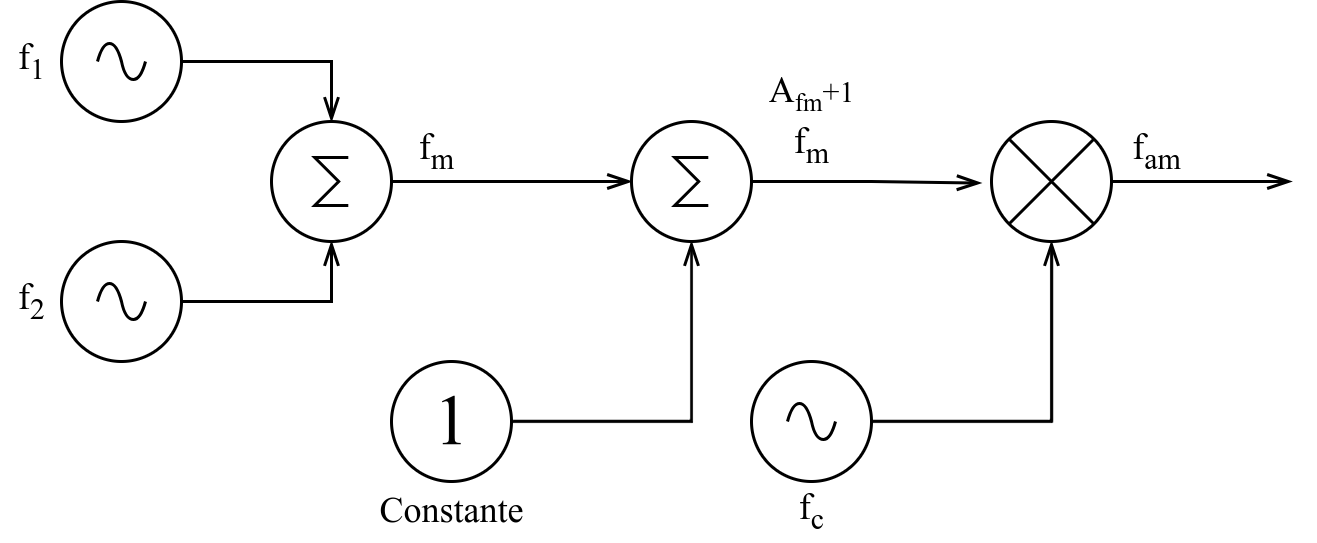
\includegraphics[width=400pt]{images/desarrollo/cod_mod.png}
  \caption{Codificador y Modulador}
  \label{fig:bloques_cod_mod}
\end{figure}

\subsection*{Transmisión}
La transmisión será simulada a través de un filtro pasa-banda, estableciendo las frecuencias de corte de tal forma que el ancho de banda sea el espectro audible por el oído humano, como muestra la Figura \ref{fig:bloques_txs}.

\begin{figure}[!htb]
  \centering
  
\includegraphics[width=300pt]{images/desarrollo/canal.png}
  \caption{Transmisión}
  \label{fig:bloques_txs}
\end{figure}

\subsection*{Demodulador}
Para demodular la señal, basta con realizar nuevamente el producto con la señal portadora. Como resultado obtenemos la frecuencia moduladora (que es la señal codificada, suma de las frecuencias que componen a un digito específico) como muestra la Figura \ref{fig:bloques_demod}. Luego debemos aplicar un filtro pasa bajos para limpiar la señal de ruidos que puedan haberse introducido, entre esos, algunos vestigios de la señal portadora.

\begin{figure}[!htb]
  \centering
  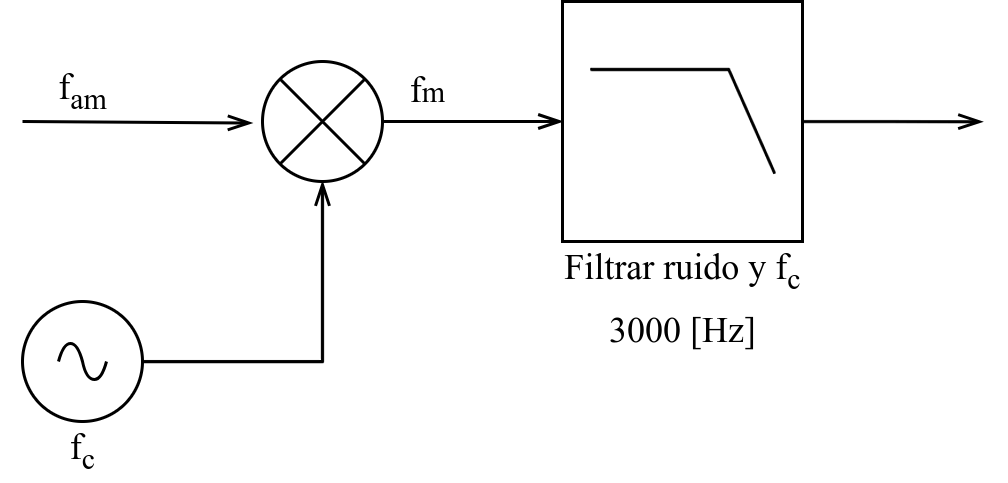
\includegraphics[width=350pt]{images/desarrollo/demod.png}
  \caption{Transmisión}
  \label{fig:bloques_demod}
\end{figure}

\subsection*{Decodificador}
El bloque decodificador es el más complejo de todos, ya que este tiene la lógica para detectar las señales que componen la señal codificada. Como ya vimos en la Figura \ref{fig:diagrama_bloques_decod}, necesitamos 7 filtros pasa-banda para aislar cada una de las frecuencias de la matriz \gls{dtfm}, luego viene la matriz decodificadora. En la Figura \ref{fig:bloques_decod} vemos una simplificación de cómo estaría compuesta esta lógica de decodificación. Cada salida de control es una compuerta AND que se activara cuando sus dos entradas se encuentren activas (o en "1" lógico). Entonces cada compuerta representa la combinación de tonos para detectar cuál fué el digito enviado.

\begin{figure}[!htb]
  \centering
  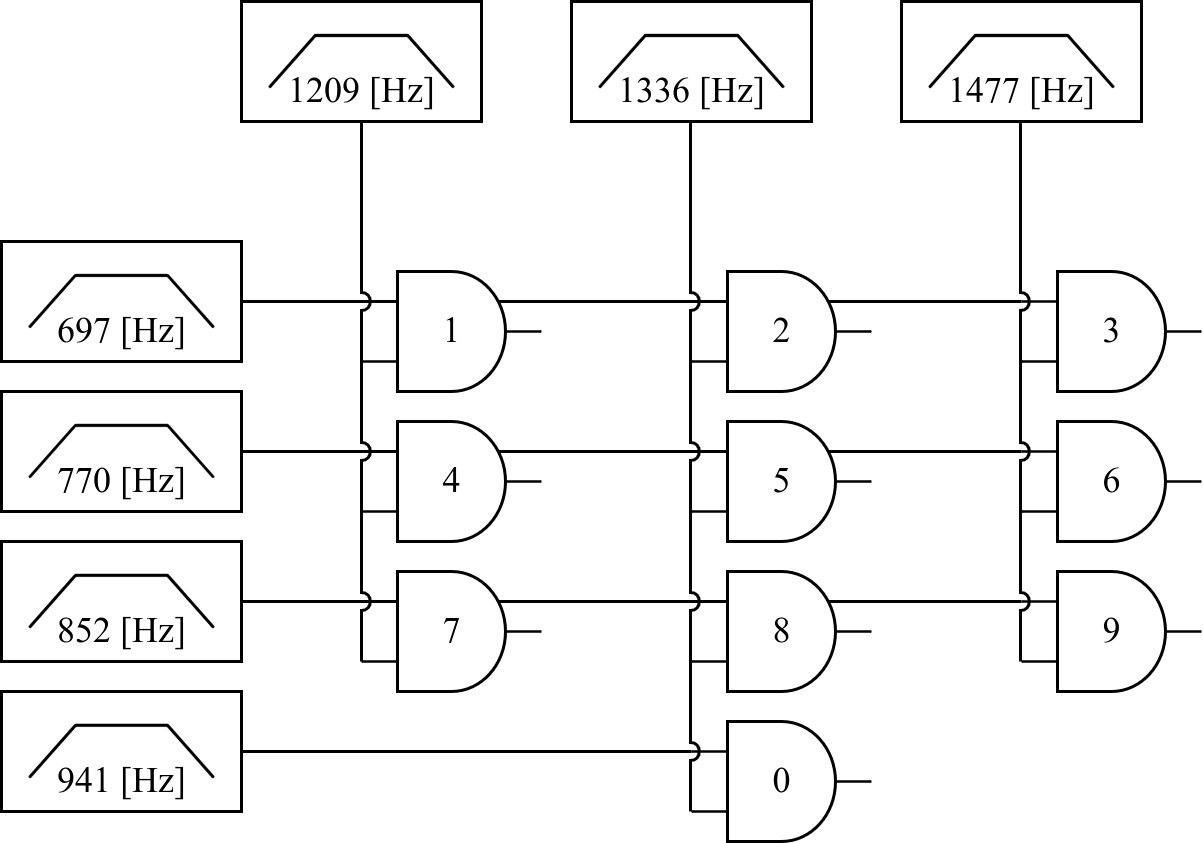
\includegraphics[width=350pt]{images/desarrollo/decod.png}
  \caption{Decodificador}
  \label{fig:bloques_decod}
\end{figure}

\section{Diseño}
Como mencionamos en la sección anterior, para poder implementar los filtros digitales del banco de filtros (bloque decodificador) necesitamos librerías de MATLAB para generarlos, ya que estos filtros serán de alto orden lo que es engorroso para el cálculo analítico. Para hacer uso de estas librerías se crearon 2 \textit{scripts} con el objetivo de automatizar la generación de los filtros en base a parámetros de entrada. En el Código \ref{code:banco_decodificador} podemos ver que se encarga de calcular las frecuecias de corte (inferior y superior) para cada frecuencia central provista, bajo una determinada frecuencia de muestreo y orden específico, esto para el banco de filtros del decodificador. Además de eso, también podemos ver que genera las gráficas para analizar la respuesta en frecuencia de cada filtro, como muestra la Figura \ref{fig:banco_filtros_resp_frec}. Luego en el Código \ref{code:algoritmo_principal} tenemos el algorítmo principal, el cual establece las especificaciones generales del sistema, llama a la función para crear el banco de filtros y además crea el resto de los filtros involucrados como el que representa el canal de transmición y el filtro para eleminar la portadora del espectro de trabajo (en la fase de demodulación).

Se puede notar en el Código \ref{code:algoritmo_principal} que establecemos el orden de los filtros en 6 (para pasa-bajos y/o pasa-altos; se interpreta 12 para pasa-banda). Este valor arbitrario, contrario a los cálculos analíticos del capítulo anterior, es empírico; durante varias pruebas de simulación, los filtros pasa-banda de alto orden (20 aproximadamente) demostraban comportamientos inesperados y no concluyentes a la hora de filtrar señales específicas. Por eso, luego de varias pruebas encontramos que el orden 6 era suficiente para realizar la simulación con resultados favorables y realistas.

Es de suponer que estos filtros diseñados por matlab son estables, sin embargo no dejamos pasar la oportunidad de hacer un análisis de cada uno. Para realizarlo utilizamos una función cuyo código se puede ver en el Apendice \ref{code:script_analisis}. El resultado se puede ver en los siguientes apendices:

\begin{enumerate}
  \item Filtro pasa-banda centrado en 697 [Hz]: Apendice \ref{fig:analisis_697}.
  \item Filtro pasa-banda centrado en 770 [Hz]: Apendice \ref{fig:analisis_770}.
  \item Filtro pasa-banda centrado en 852 [Hz]: Apendice \ref{fig:analisis_852}.
  \item Filtro pasa-banda centrado en 941 [Hz]: Apendice \ref{fig:analisis_941}.
  \item Filtro pasa-banda centrado en 1209 [Hz]: Apendice \ref{fig:analisis_1209}.
  \item Filtro pasa-banda centrado en 1336 [Hz]: Apendice \ref{fig:analisis_1336}.
  \item Filtro pasa-banda centrado en 1477 [Hz]: Apendice \ref{fig:analisis_1477}.
\end{enumerate}

También se pueden ver los Polos y Ceros de cada filtro en el Apendice \ref{sec:pz}.

\begin{figure}[H]
  \lstinputlisting[
    language=Octave,
    caption={Banco Decodificador},
    label={code:banco_decodificador}
  ]{matlab/desarrollo/banco_decodificador.m}
\end{figure}

\begin{figure}[!htb]
  \centering
  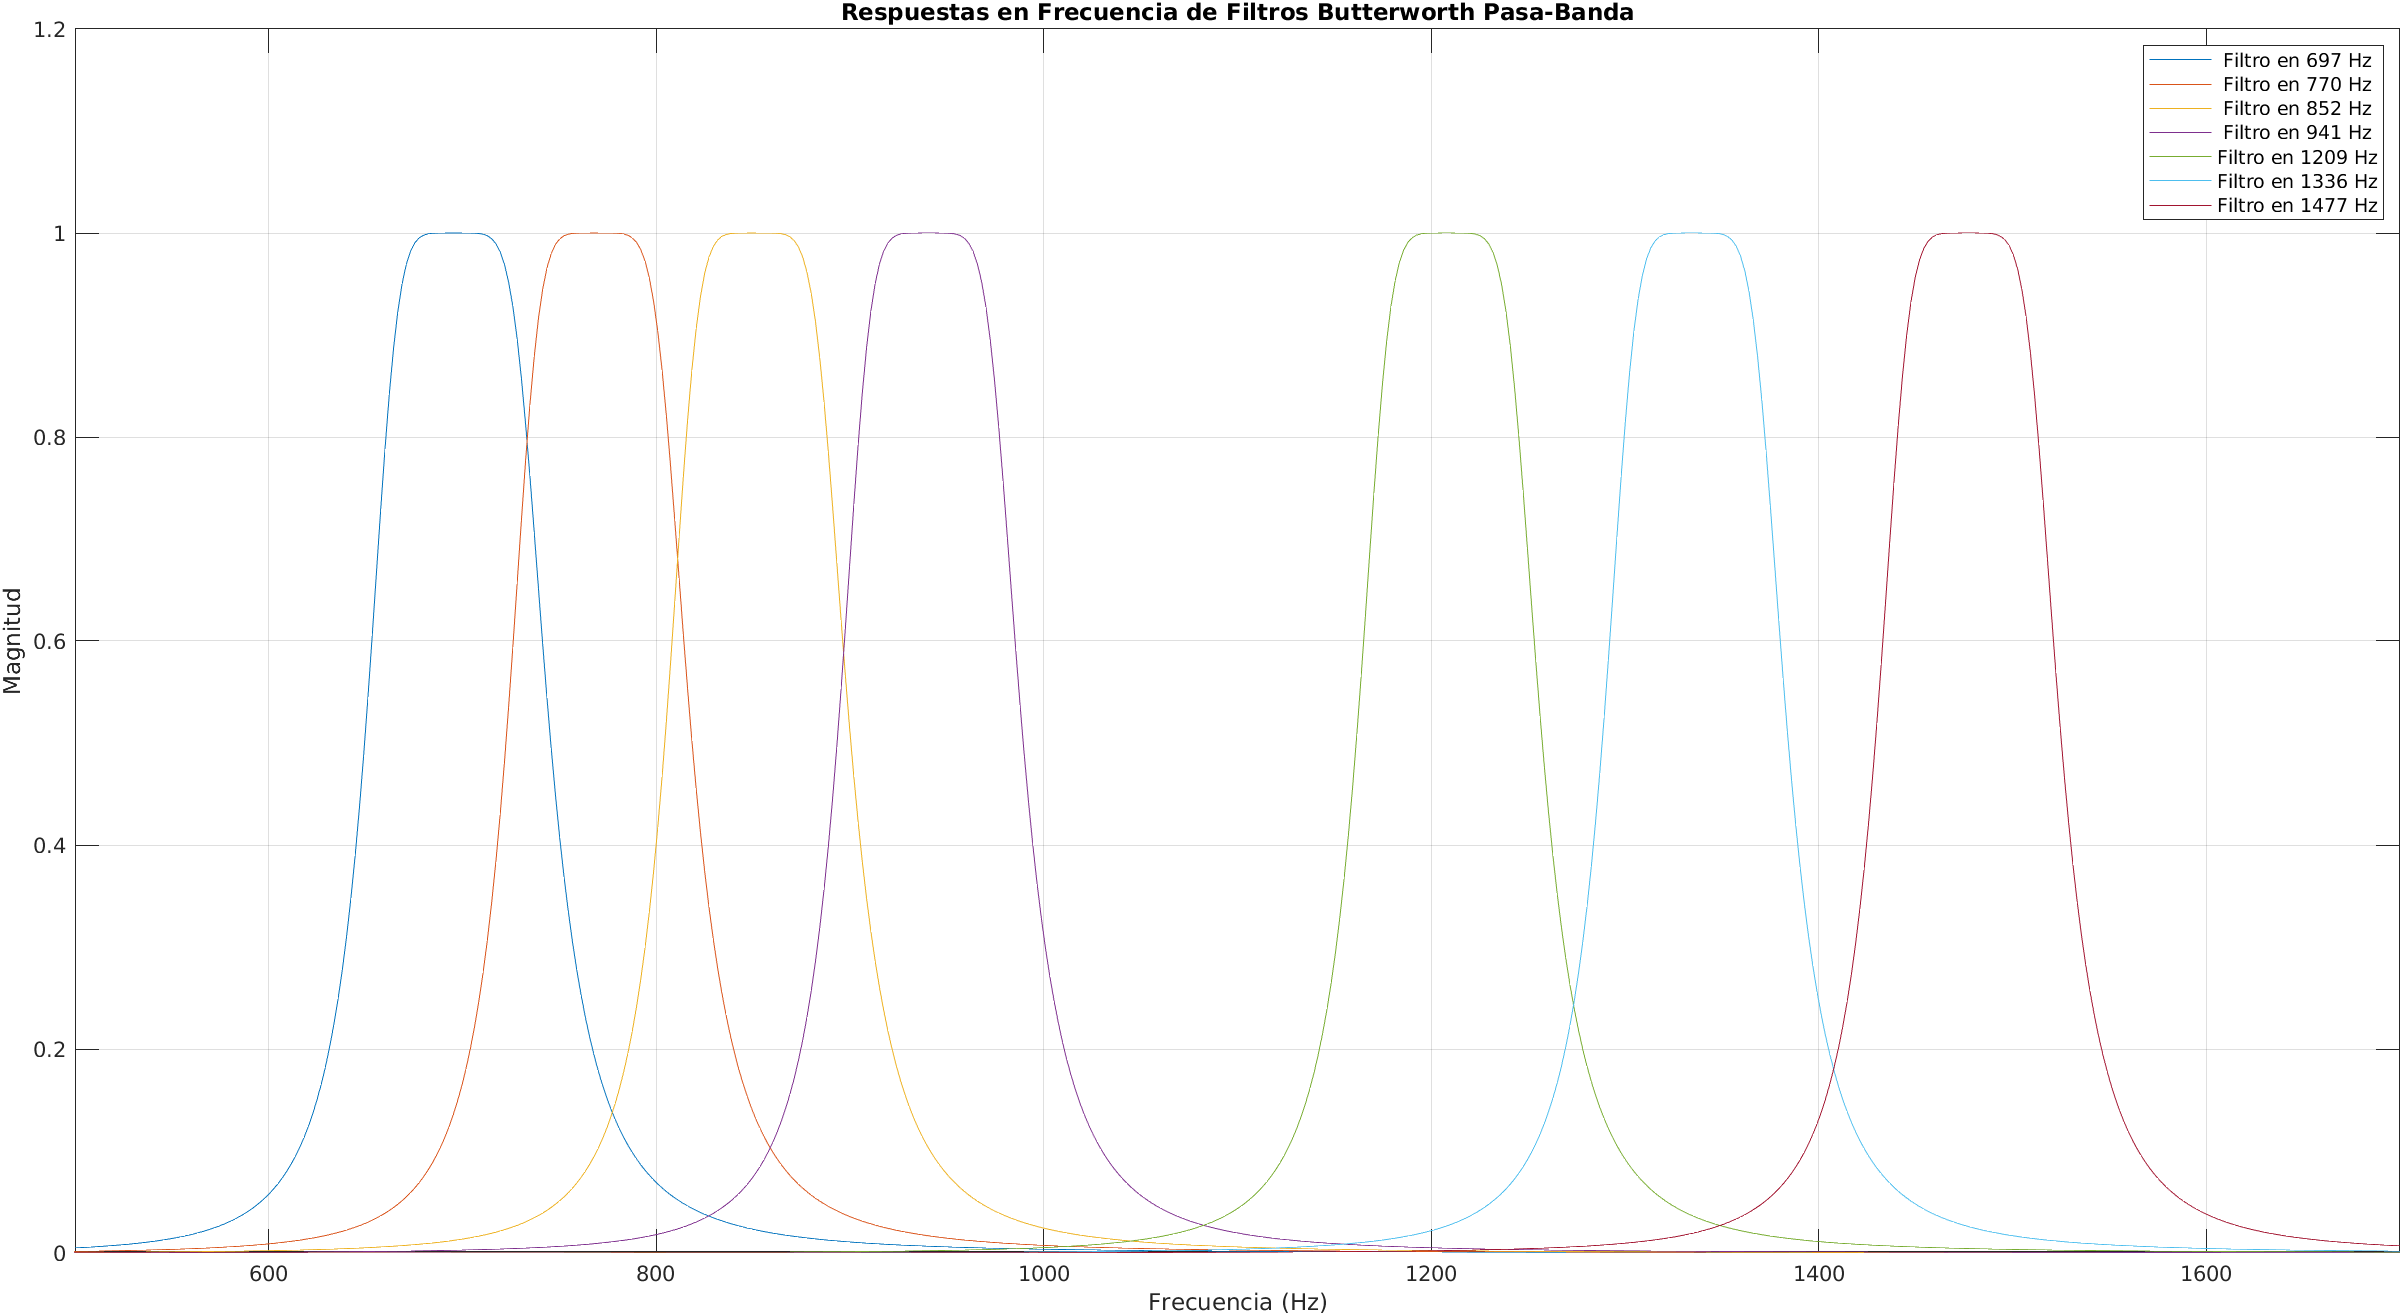
\includegraphics[width=\linewidth]{images/desarrollo/freq_filtros.png}
  \caption{Respuesta en frecuencia del Banco de Filtros}
  \label{fig:banco_filtros_resp_frec}
\end{figure}

\begin{figure}[H]
  \lstinputlisting[
    language=Octave,
    caption={Algorítmo principal},
    label={code:algoritmo_principal}
  ]{matlab/main.m}
\end{figure}

\section{Prototipo}
En base a los resultados obtenidos de los \textit{scripts} diseñamos el sistema completo, en los que cada bloque se alimenta de los datos resultantes. En la Figura \ref{fig:bloques_modem} podemos ver los bloques intervinientes en la primera parte del sistema, esta incluye la selección de los tonos (inferior y superior) para luego sumarlos y lograr la codificación \gls{dtfm} del número 5 en este caso. Luego pasamos a los bloques intervinientes en la modulación AM de las señales, sumando antes una constante 1 para poder realizar el producto con la señal portadora. Una vez obtenida la señal modulada en AM, esta se transmite por el canal de modulación, que según las especificaciones tiene el ancho de banda del espectro audible por el oído humano. Luego llega a la etapa de demodulación, en la que la señal se vuelve a batir (producto) con la portadora, y el resultado es una señal que tiene una componente en la frecuencia de la portadora y debe ser filtrada, por ello utilizamos un filtro pasa-bajos con frecuencia de corte 3[kHz]. Pasado este filtro, la señal obtenida es casi identica a la sumatoria de los dos tonos.

La segunda parte del sistema comprende la decodificación \gls{dtfm} a través de un banco de filtros y una matriz decodificadora, como se muestra en la Figura \ref{fig:bloques_codec}. Primero debemos aislar las señales por tonos diferenciados, esto lo hace el banco de filtros digitales. Cada uno de estos es un filtro pasa-banda con frecuencia central en uno de los 7 tonos, de esta forma logramos aislar cada señal. Dado que estas son sinusoidales, necesitamos calcular el valor efectivo de las mismas para poder operar lógicamente ellas, entonces se coloca un bloque que realiza el cálculo. Luego, el valor obtenido es un número decimal, del cual nos interesa la parte entera, ya que con este dato vamos a validar la amplitud con la que la señal sale del filtro. La razón de hacer este procedimiento es que para poder comparar lógicamente las señales presente para determinar qué tono fue codificado y enviado, lo cual se explica a continuación.

\begin{figure}[!htb]
  \centering
  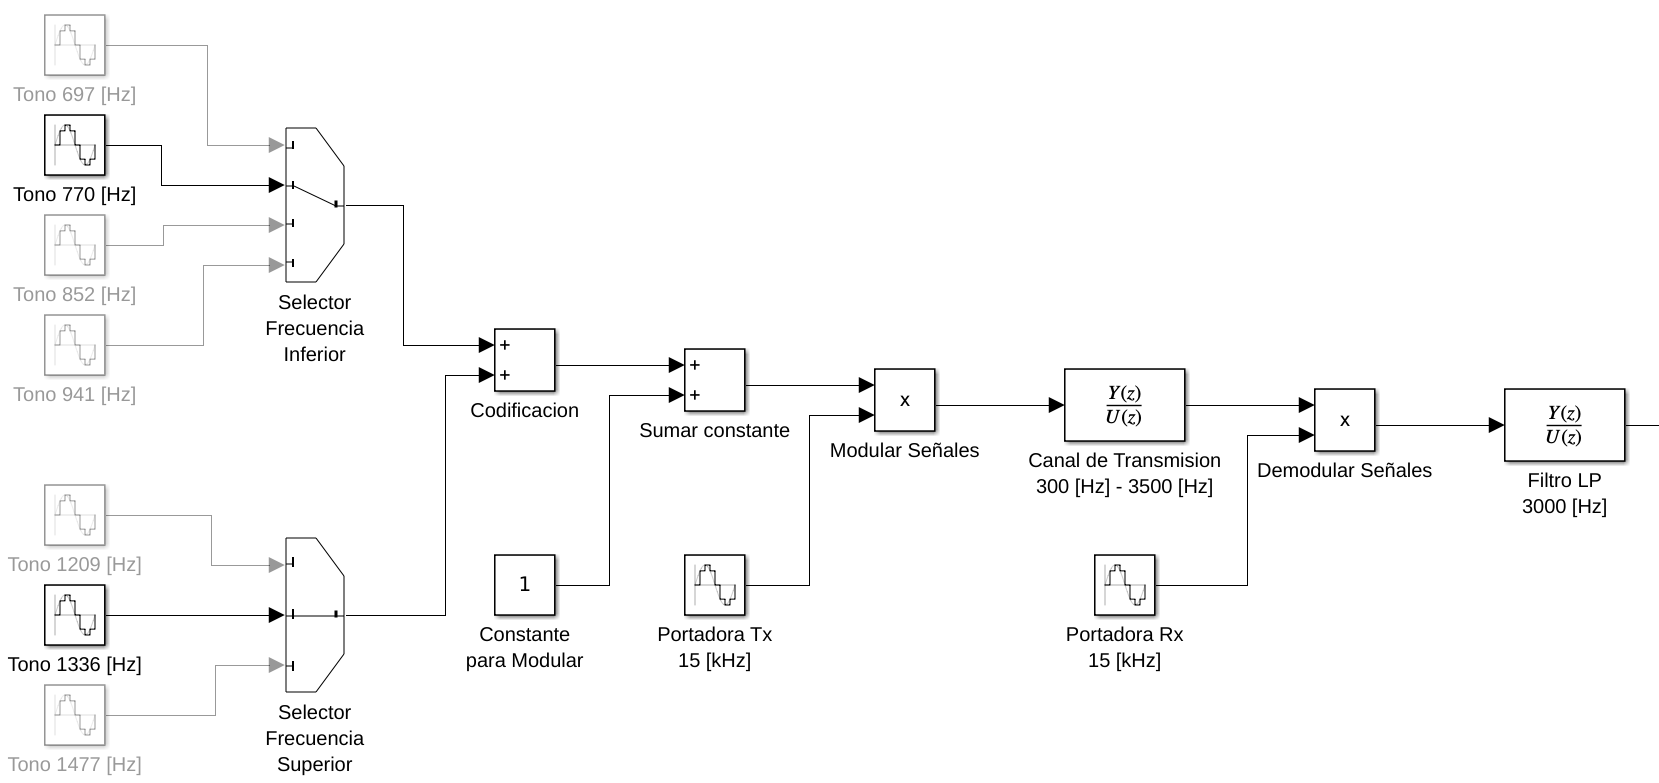
\includegraphics[width=\linewidth]{images/desarrollo/modem.png}
  \caption{Codificación, Modulación, Transmisión y Demodulación}
  \label{fig:bloques_modem}
\end{figure}

\begin{figure}[!htb]
  \centering
  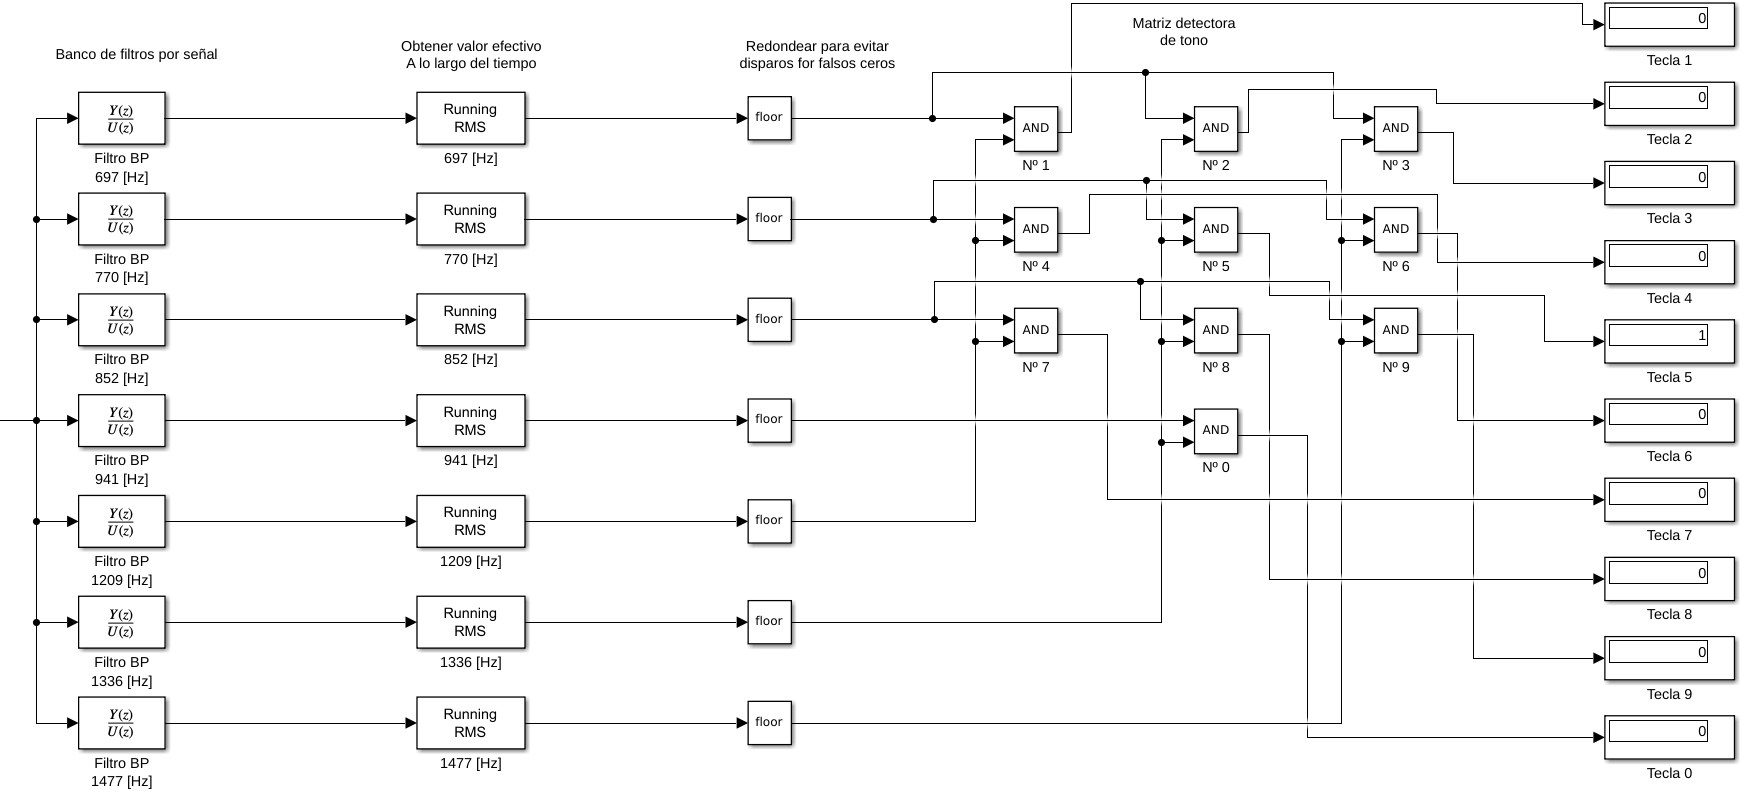
\includegraphics[width=\linewidth]{images/desarrollo/codec.png}
  \caption{Banco de filtros y Decodificador}
  \label{fig:bloques_codec}
\end{figure}

La matriz decodificadora se compone de bloques de operación lógica AND. La salida de este bloque será 1 si y solo si ambas entradas son diferentes a 0\footnote{En el álgebra booleana aplicada en sistemas de control, todo valor igual a 0 se toma como "Falso", mientras que cualquier valor distinto de 0, por más infinitesimal que sea, es "Verdadero"}. Como los filtros anteriores son de orden relativamente bajo, es posible que al tratar las señales dejen pasar vestigios de la otra señal en la codificación pero con mucha menor amplitud. El valor efectivo de este resultado puede ser muy bajo, infinitesimal, del orden de $10^{-2}$, pero no 0 y por consiguiente el operador lógico lo tomará como válido y puede disparar falsos valores. Por esa razón debemos tomar la parte entera del valor eficaz, para garantizar que solo se debe tomar como válida a las señales que realmente son de la misma frecuencia que la frecuencia central de cada filtro.

\section{Simulación}
Para llevar a cabo la simulación vamos a considerar una serie de escenarios posibles, en los que se diferencia mayormente la confiabilidad en el canal de transmisión. Es decir, confiaremos en los bloques de control ya que son implementados a través de sistemas computacionales, pero el medio de transmisión es analógico y su eficacia depende de muchos factores físicos. Este se puede ver alterado de diversas maneras haciendo que parte de la información se pierda o corrompa. Para ello vamos a probar los siguientes escenarios:

\begin{enumerate}
  \item El canal de transmisión es del tipo AWG-24 de menos de 200 [m] de largo, cuyo ancho de banda es de 1 [MHz].
  \item El canal de transimsión es extenso y tiene el ancho de banda del espectro audíble por los humanos.
  \item El mismo canal anterior presenta fallas atenuando en diferentes frecuencias dentro del espectro de tonos \gls{dtfm}
\end{enumerate}

\subsection{Ancho de banda Extendido - 1 [MHz]}
A los efectos prácticos, un canal de 1 [MHz] de ancho de banda bien podría ser considerado un canal ideal, lo que en la simulación equivaldría a no poner un filtro represtantivo del canal de transmisión. Eso significa que toda la señal que sale del modulador llega al demodulador. Sin embargo, realizaremos la simulación utilizando un filtro en el canal para obtener resultados lo más realista posible.

Dado de que la frecuencia de muestreo es de 44 [kHz], y por el Teorema de Nyquist-Shannon, la máxima frecuencia a muestrear debería ser menor o igual a la mitad de la frecuencia de muestreo. Por ello vamos a tomar que el canal tiene un ancho de banda que va desde 0 [Hz] hasta 20000 [Hz]. Este será implementado con un filtro Butterworth de 2do orden pasa-bajos para obtener para obtener una respuesta plana en la banda de paso.

Para realizar esta simmulación, haremos una modificación en el Código \ref{code:algoritmo_principal}, cambiaremos la banda de paso del filtro del canal con los valores \lstinline{butter(2, 22000 / (Fs / 2))}, ejecutamos el \textit{script} y probaremos enviar el número 1.

\begin{figure}[!htb]
  \centering
  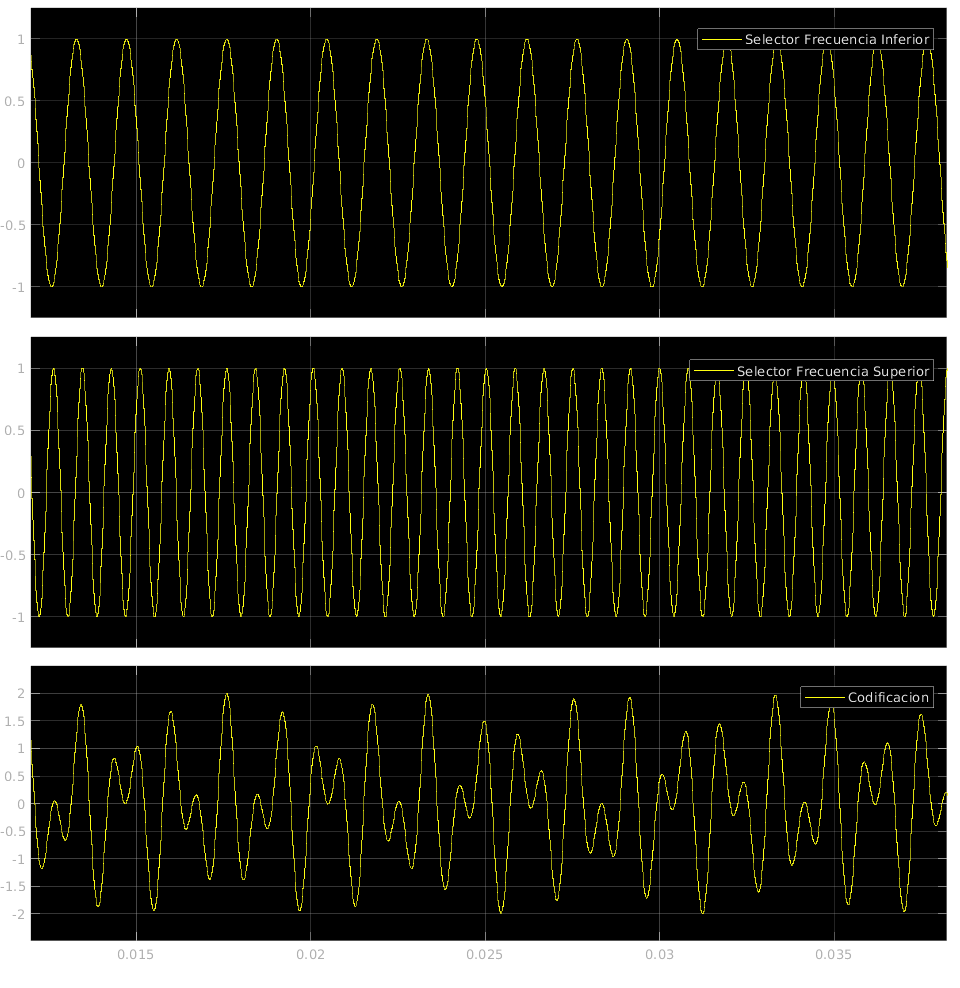
\includegraphics[width=\linewidth]{images/simulacion/extendido/cod.png}
  \caption{Codificación del número 1}
  \label{fig:sim_cod}
\end{figure}

En la Figura \ref{fig:sim_cod} podemos observar la etapa de codificación. Las 2 primeras señales son la frecuencia inferior y superior que componen al número 1 (697 [Hz] y 1209 [Hz]), y la tercera es el resultado de sumar ambas señales.

\begin{figure}[!htb]
  \centering
  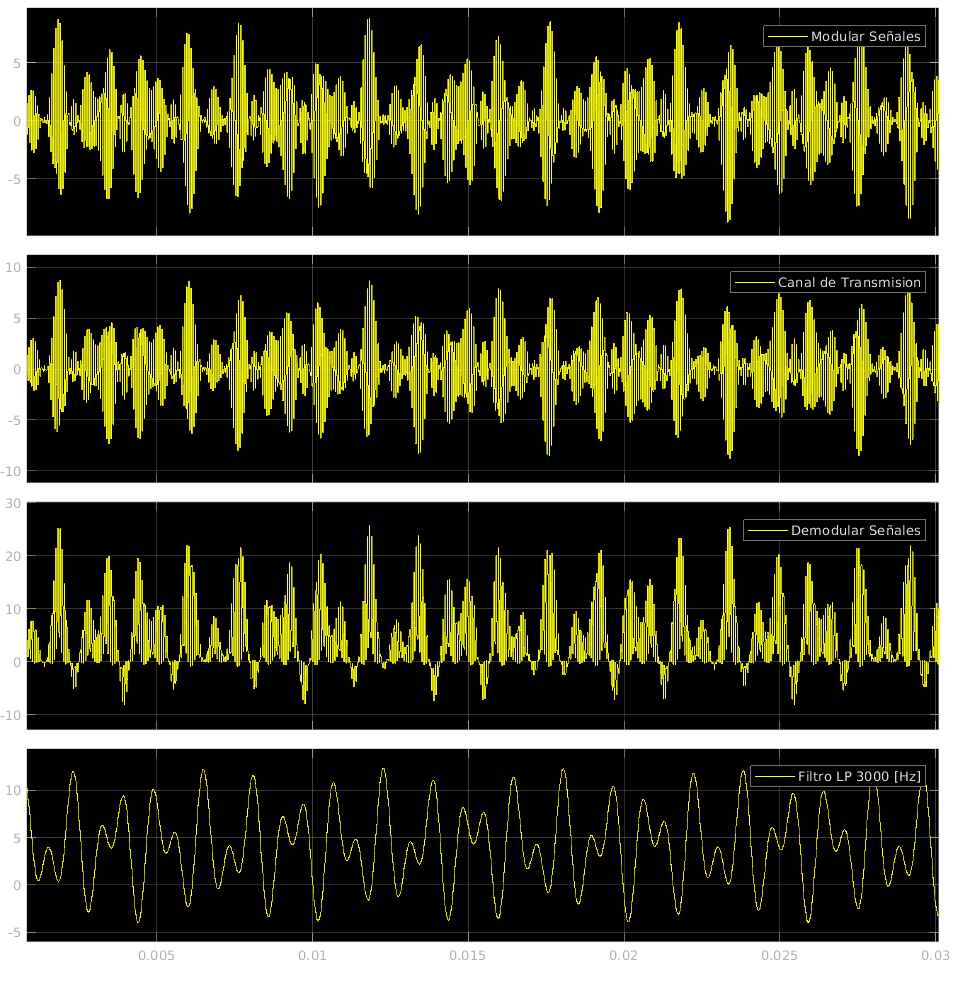
\includegraphics[width=\linewidth]{images/simulacion/extendido/modem.png}
  \caption{Modulación, Transmisión y Demodulación}
  \label{fig:sim_modem}
\end{figure}

En la Figura \ref{fig:sim_modem} tenemos 4 muestras. La primera es la señal modulada, es decir la portadora modulada por la señal codificada del número 1. En la segunda muestra es la misma señal pero a través del filtro represtantivo del canal. Podemos notar que son similares pero se encuentran desfasadas, y esto se debe al filtro en sí. También podemos obervar que la señal no tuvo perdidas de ganancia, mantiene la amplitud con la que salío del modulador. En la tercera muestra vemos la señal luego de ser demodulada, en la que podemos ver que no tiene la forma de la señal codificada, y esto es porque aún tiene una componente de la frecuencia de la señal portadora. En la cuarta muestra vemos que la señal ya tiene la forma de la señal codificada, esto es porque pasó por el filtro pasa-bajos a 3000 [Hz], eliminando así dicha componente.

\begin{figure}[!htb]
  \centering
  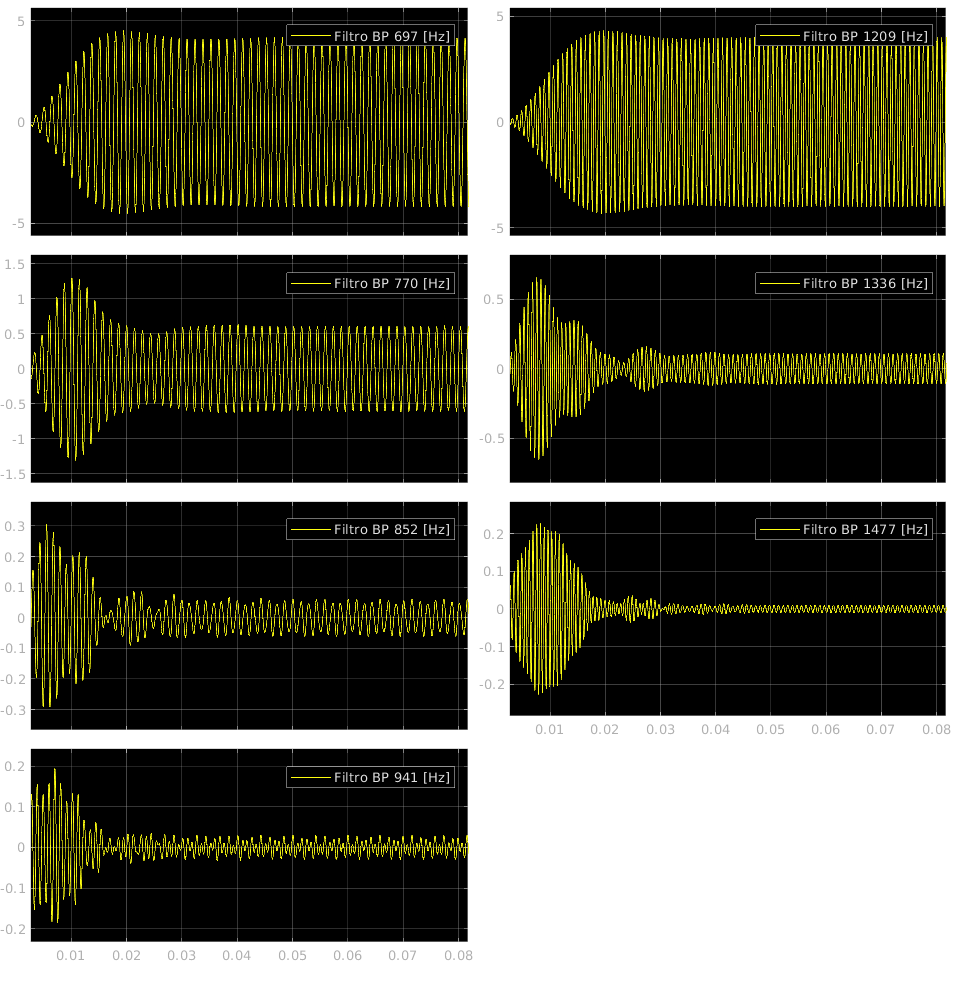
\includegraphics[width=\linewidth]{images/simulacion/extendido/bank.png}
  \caption{Salida del Banco de Filtros}
  \label{fig:sim_bank}
\end{figure}

Una vez tratada y obtenida la señal deseada, puede pasar al banco de filtros para poder aislar las señales que componen la codificación. En la figura \ref{fig:sim_bank} obervamos la respuesta de cada filtro a la señal, y podemos notar rápidamente que en los filtros de 697 [Hz] y 1209 [Hz] las salidas son con mayor intensidad (porque son las que realmente buscamos aislar), mientras que en las otras se atenúa considerablemente. En algunos filtros se atenúa más que otros y esto se debe al solapamiento que tienen los filtros debido a la proximidad de las frecuencias en cuestión.

\begin{figure}[!htb]
  \centering
  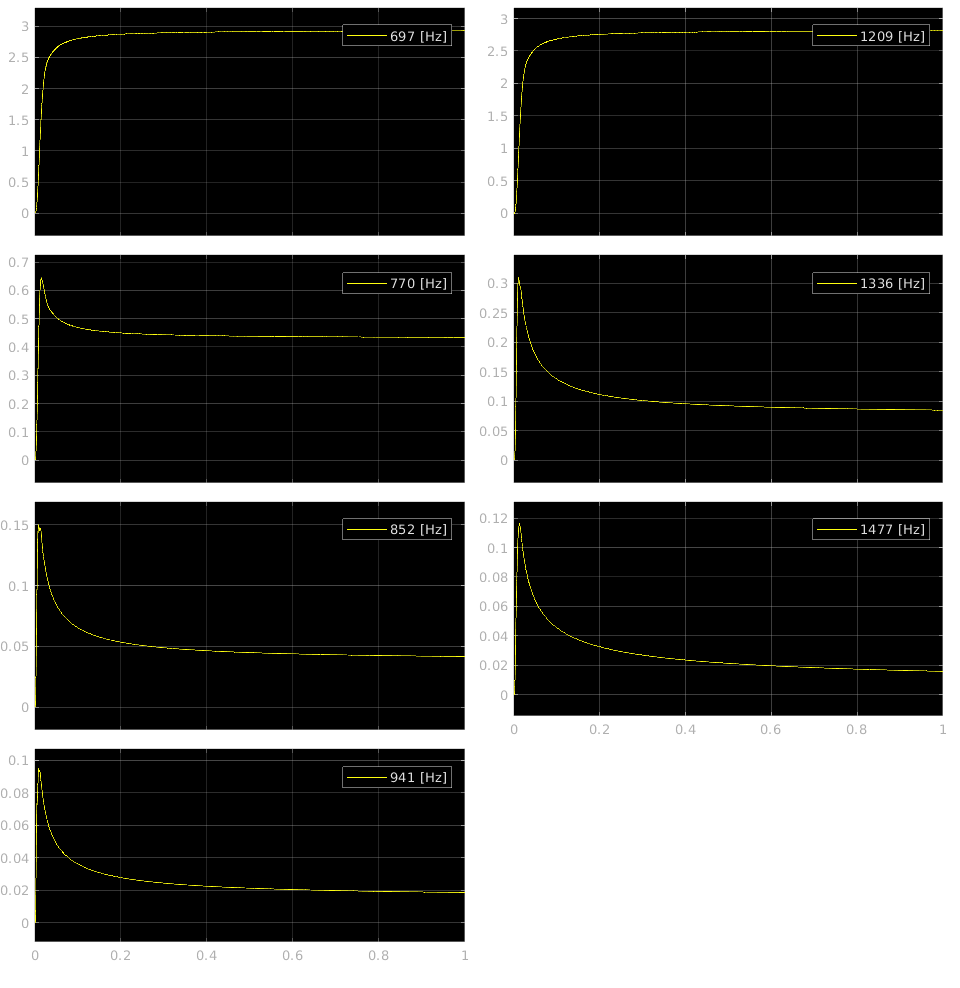
\includegraphics[width=\linewidth]{images/simulacion/extendido/rms.png}
  \caption{Valor Eficaz del Banco de Filtros}
  \label{fig:sim_rms}
\end{figure}

Luego de aislar las señales, necesitamos obtener el valor eficaz de cada salida. En la Figura \ref{fig:sim_rms} obervamos las salidas de cada bloque RMS y claramente de los filtros que no que no son de interés se obtiene valores muy pequeños en contraste con los 2 que sí nos interesa. El paso siguiente es obtener el valor númerico de esas salidas para obtener solamente la componente entera, que en nuestra simulación determina que esa señal está activa.

\begin{figure}[!htb]
  \centering
  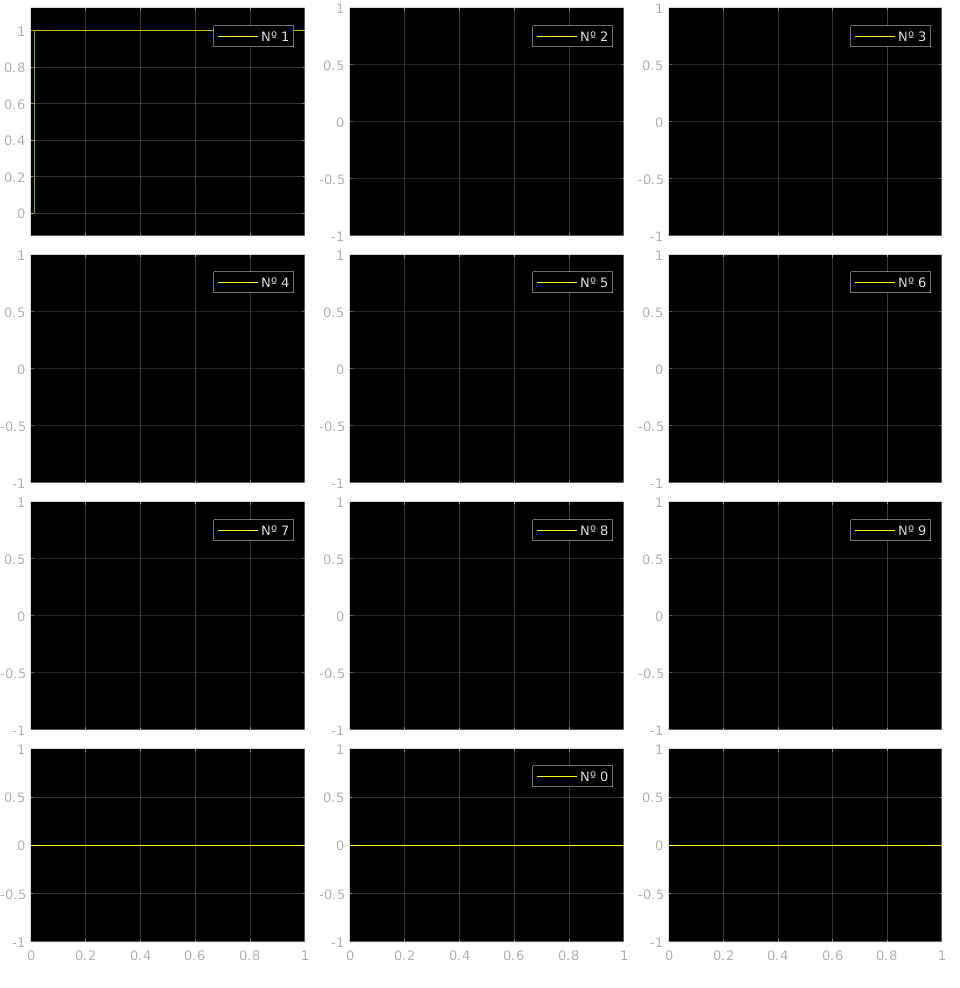
\includegraphics[width=\linewidth]{images/simulacion/extendido/decod.png}
  \caption{Decodificación de las Señales}
  \label{fig:sim_decod}
\end{figure}

Para finalizar obersvamos las salidas de las compuertas lógicas de la matriz decodificadora. En la Figura \ref{fig:sim_decod} tenemos cada muestra dispuesta como un teclado numérico, con su etiqueta correspondiente. Notamos que la muestra del número 1 es la única que tiene valor alto (1 lógico), mientras que las otras están en 0\footnote{En algunas muestras no se logra ver la señal debido a fallas en la renderización de la gráfica, pero si fueran 1 se verían como la primera muetra}. Para mejorar la visualización del funcinamiento, en la Figura \ref{fig:sim_sim} se muestran los Visores al final del sistema, los cuales muestran los valores de las señales de la matriz decodificadora, y nuevamente, vemos que todas están en 0 con la excepción de la tecla número 1.

\begin{figure}[!htb]
  \centering
  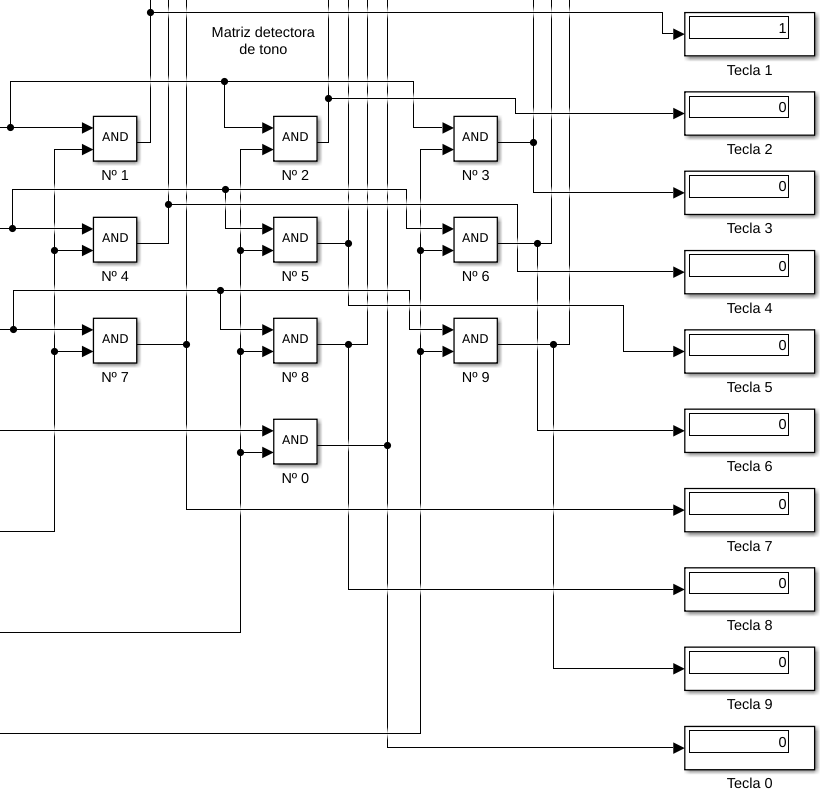
\includegraphics[width=400pt]{images/simulacion/extendido/sim.png}
  \caption{Visor de la Simulación}
  \label{fig:sim_sim}
\end{figure}


\subsection{Ancho de banda Reducido - 3 [kHz]}
Para esta simulación, modificamos nuevamente el Código \ref{code:algoritmo_principal} para que vuelva a operar con el canal real, establecido entre 300 [Hz] y 3500 [Hz]. Por motivos de simplicidad la simulación la vamos a analizar directamente desde el canal, ya que la etapa de codificación no se modifica.

Para empezar, vamos a hacer un análisis de la estabilidad del canal ya que este ahora es diferente al canal "ideal" del apartado anterior. Para ello hicimos uso del Código \ref{code:script_analisis} y obtuvimos los resultados que se muestran en la Figura \ref{fig:real_chan}. Se puede observar que los polos indican que el filtro es estable, sumado a que la respuesta al impulso y al escalón también lo reafirman. Pero lo que llama la atención aquí es la respuesta en frecuencia del filtro. Es de esperarse que la curva tenga esa forma, ya que para eso fue diseñado, pero vemos también que está filtrando componentes de alta frecuencia, casualmente entre ellas se encuentra la señal portadora. Vamos a analizar si esto representa un problema para la simulación.

\begin{figure}[!htb]
  \centering
  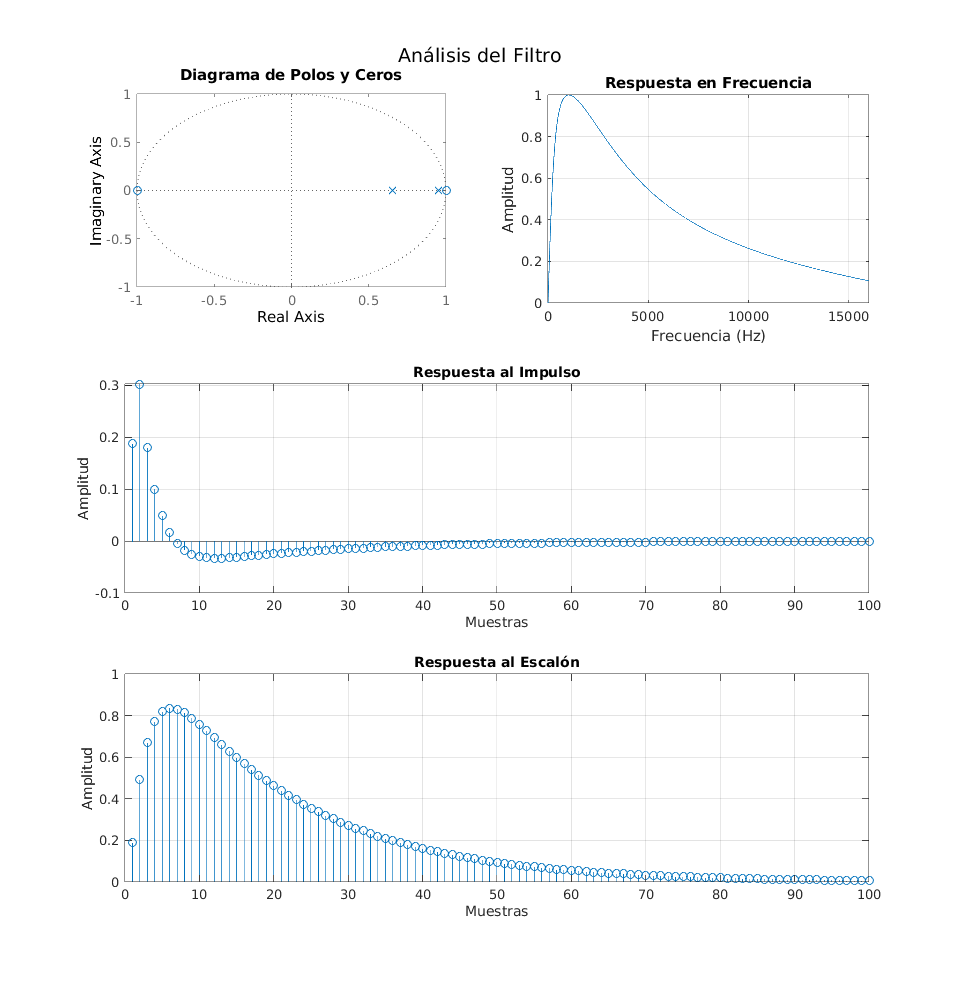
\includegraphics[width=\linewidth]{images/simulacion/reducido/chan.png}
  \caption{Estabilidad del Canal}
  \label{fig:real_chan}
\end{figure}



\begin{figure}[!htb]
  \centering
  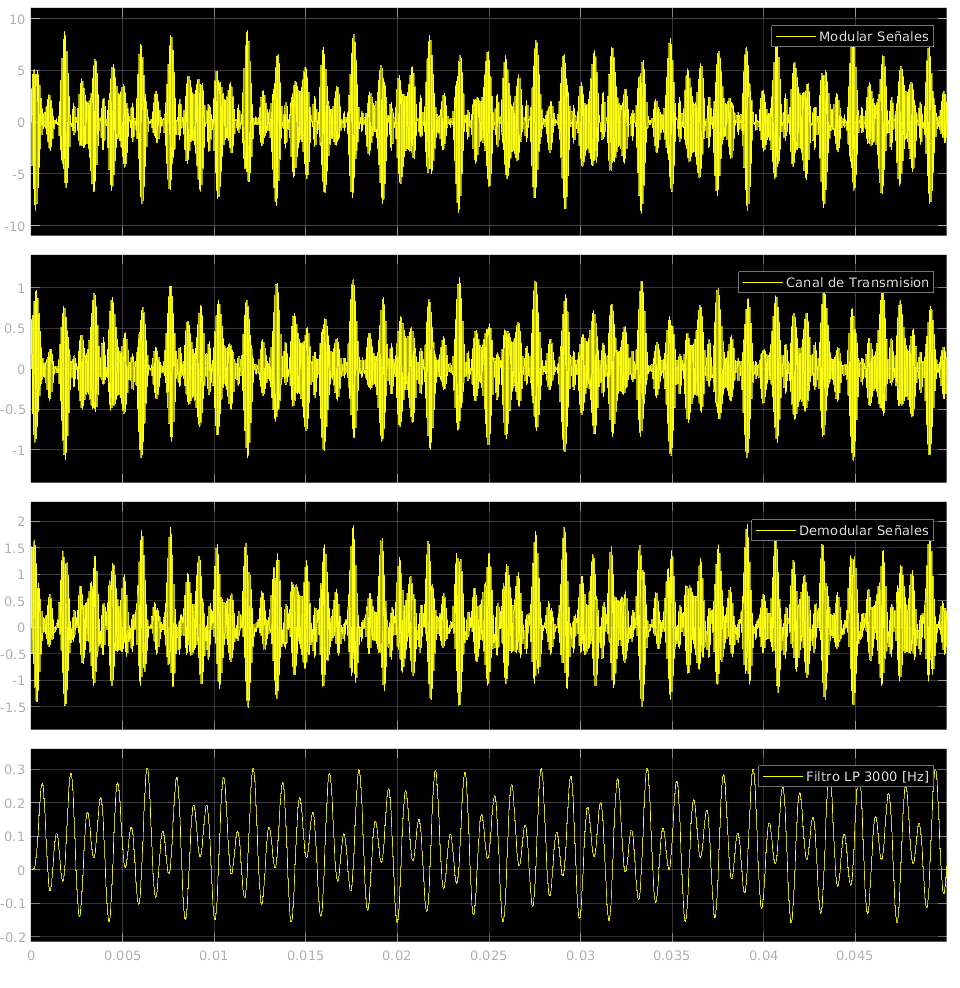
\includegraphics[width=\linewidth]{images/simulacion/reducido/modem.png}
  \caption{Modulación, Transmisión y Demodulación}
  \label{fig:real_modem}
\end{figure}

\pagebreak

En la Figura \ref{fig:real_modem} vemos que al pasar por el canal, la señal se ve drásticamente atenuada (casi 10 veces menos) lo cual ya puede significar un problema considerando que en el ejemplo anterior esto no pasaba. Luego de pasar por el demodulador, la señal parece que no sufrió ningún cambio, esto pude ocurrir porque la componente con mayor amplitud (la portadora) ha sido filtrada, con lo cual la demodulación ya no tiene sentido. Y luego pasando por el filtro que estaba destinado a filtrar la portadora, la señal pierde más ganancia. Todo parece indicar que el sistema no va a funcionar correctamente debido a que la señal llega con poca fuerza al banco de filtros.

\begin{figure}[!htb]
  \centering
  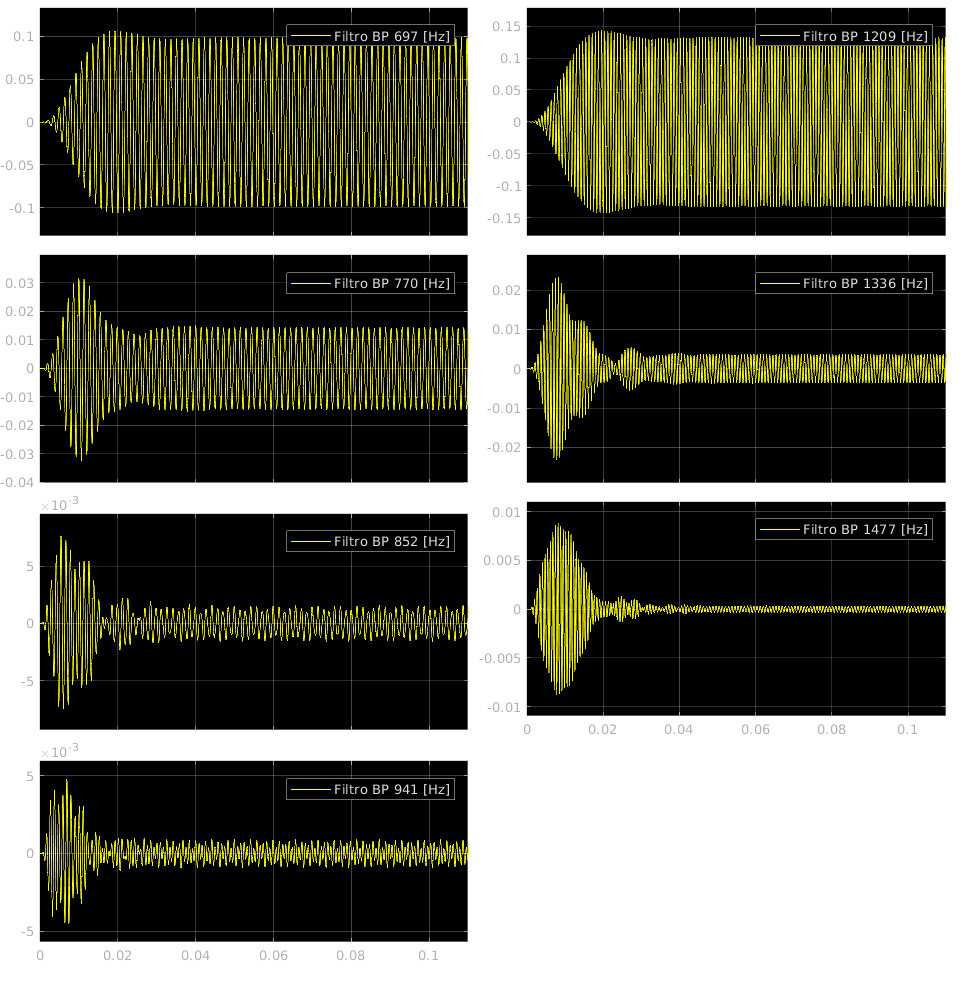
\includegraphics[width=\linewidth]{images/simulacion/reducido/bank.png}
  \caption{Salida del Banco de Filtros}
  \label{fig:real_bank}
\end{figure}

\begin{figure}[!htb]
  \centering
  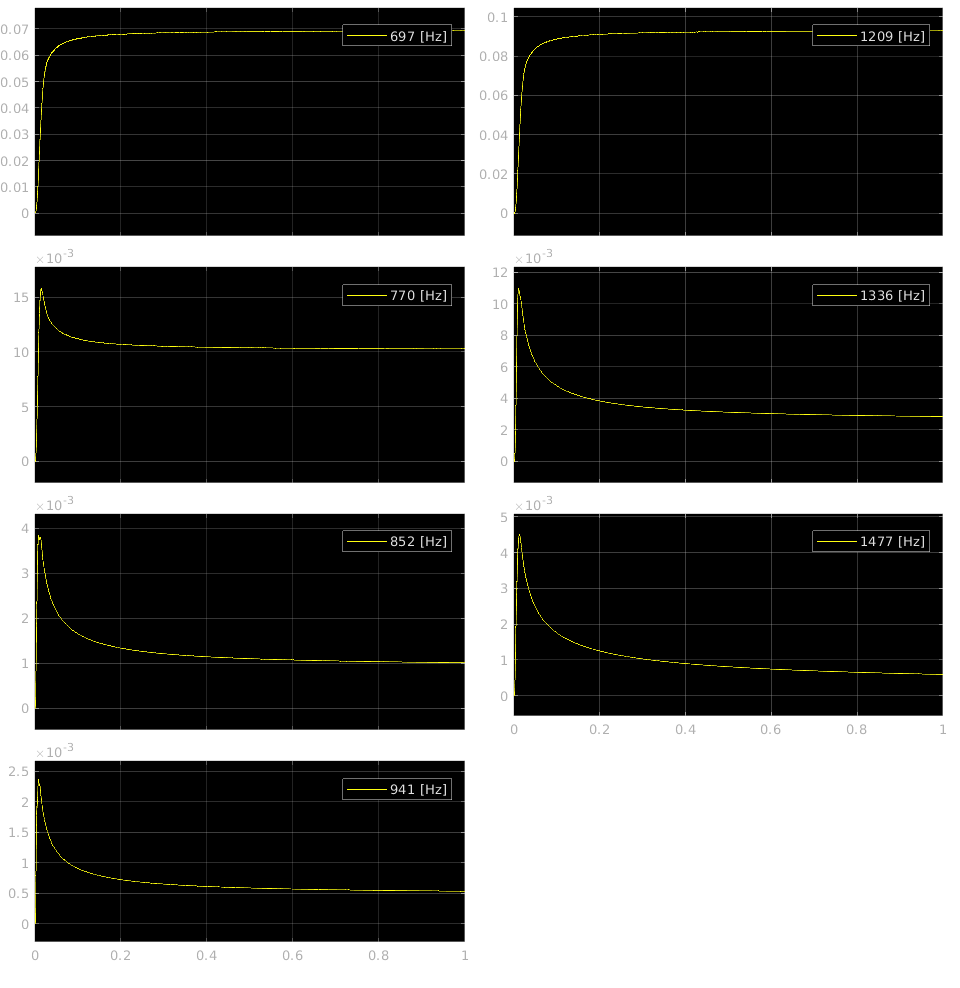
\includegraphics[width=\linewidth]{images/simulacion/reducido/rms.png}
  \caption{Valor Eficaz del Banco de Filtros}
  \label{fig:real_rms}
\end{figure}

\pagebreak

Al pasar por el banco de filtros, como muestra la Figura \ref{fig:real_bank}, podemos notar que las señales son correctamente aisladas. Es decir que la señal codificada se puede detectar, pero estas tiene muy poca amplitud. Por consiguiente, el valor eficaz será aún menor y numericamente ninguna señal no conseguirá pasar la unidad (en magnitud), como se puede ver en la Figura \ref{fig:real_rms}.

\begin{figure}[!htb]
  \centering
  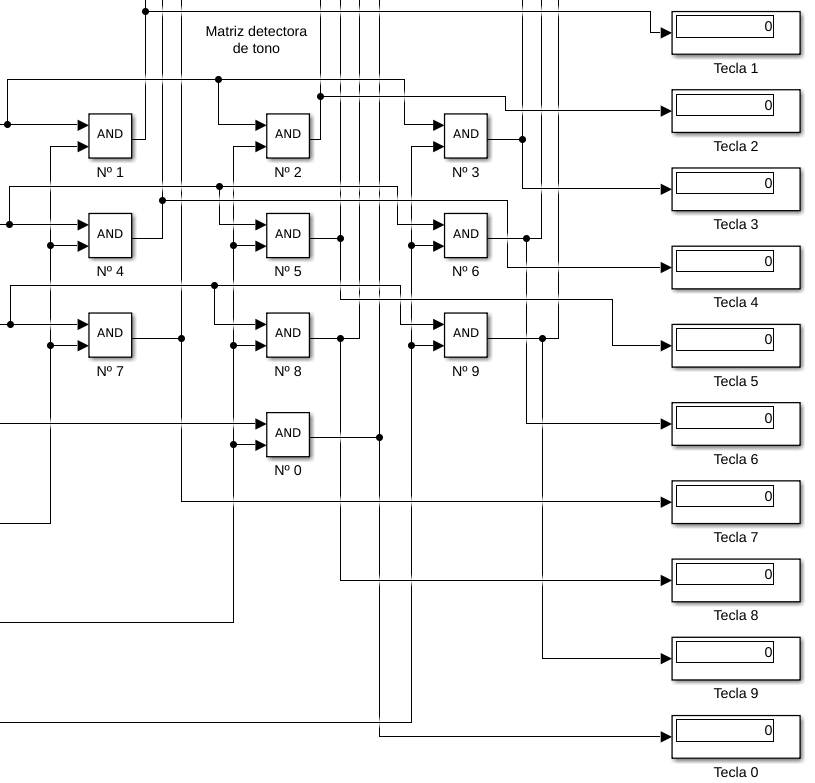
\includegraphics[width=400pt]{images/simulacion/reducido/sim.png}
  \caption{Visor de la Simulación}
  \label{fig:real_sim}
\end{figure}

\pagebreak

En consecuencia, podemos ver en el visor del sistema (Figura \ref{fig:real_sim}) que ninguna tecla se encuentra activa, ya que las señales no tienen una amplitud adecuada para lograr activar las compuertas.

Esto lo podemos analizar desde 2 puntos de vista: el sistema está mal calibrado en cuestiones de umbrales y solo necesita un ajuste (ya que las señales llegan correctamente); o bien, necesitamos aumentar la ganancia de la señal modulada enviada al canal para que el sistema siga funcionando acordementet. Empiricamente, encontramos que aumentar 20 veces la señal a la salida del modulador es suficiente para matener el sistema funcionando correctamente.

\pagebreak

Sin embargo, esto puede ser ineficiente. Claramente el canal de transimsión filtra la señal portadora entonces ¿Es realmente necesaria la modulación? Los sistemas \gls{am} están pensados para medios de transimsión en los que se pueden enviar frecuencias altas (como el aire). En un cable que tiene el ancho de banda de la voz (cable telefónico, por ejemplo) es innecesario el uso de la modulación en amplitud porque la portadora se pierde. Para este mismo sistema bastará envar la señal codificada pero con una amplitud lo suficientemente grande para que pueda a travesar el medio y pueda ser tratada a través del banco de filtros y las demás etapas.

\subsection{Canal con Fallas}

% Conclusiones
% Conclusiones
\chapter{Conclusiones}
\section{Resultados}
Aquí explicas tu metodología de investigación.

\section{Aplicaciones}

\section{Problemas en la práctica}

% Bibliografía
\bibliography{references}

% Glosario: Acrónimos
\printglossaries
\addcontentsline{toc}{chapter}{Siglas}

% Listado de figuras
\listoffigures

% Listado de tablas
\listoftables

% Listado de bloques de código
\lstlistoflistings
\addcontentsline{toc}{chapter}{Índice de bloques de código fuente}

\appendix
% Apendices
\chapter{Cálculos algebráicos}
\section{Diseño de filtro digital H(z)}

\begin{equation}
  \begin{split}
    H(\textrm{z}) & = \frac{BW \left(\frac{2}{T}\frac{(1-\textrm{z}^{-1})}{(1+\textrm{z}^{-1})}\right)}{\left(\frac{2}{T}\frac{(1-\textrm{z}^{-1})}{(1+\textrm{z}^{-1})}\right)^2 + BW \left(\frac{2}{T}\frac{(1-\textrm{z}^{-1})}{(1+\textrm{z}^{-1})}\right) + \Omega_0^2} \\
    H(\textrm{z}) & = \frac{BW \left(\frac{2}{T}\frac{(1-\textrm{z}^{-1})}{(1+\textrm{z}^{-1})}\right)}{\frac{4}{T^2}\frac{(1-\textrm{z}^{-1})^2}{(1+\textrm{z}^{-1})^2} + BW \left(\frac{2}{T}\frac{(1-\textrm{z}^{-1})}{(1+\textrm{z}^{-1})}\right) + \Omega_0^2}\ \frac{(1+\textrm{z}^{-1})^2}{(1+\textrm{z}^{-1})^2} \\
    H(\textrm{z}) & = \frac{BW \frac{2}{T} (1-\textrm{z}^{-1}) (1+\textrm{z}^{-1})}{\frac{4}{T^2} (1-\textrm{z}^{-1})^2+ BW \frac{2}{T} (1-\textrm{z}^{-1}) (1+\textrm{z}^{-1}) + \Omega_0^2 (1+\textrm{z}^{-1})^2} \\
    H(\textrm{z}) & = \frac{2 f_s \ BW  (1-\textrm{z}^{-1}) (1+\textrm{z}^{-1})}{4f_s^2 (1-\textrm{z}^{-1})^2+ 2f_s\ BW (1-\textrm{z}^{-1}) (1+\textrm{z}^{-1}) + \Omega_0^2 (1+\textrm{z}^{-1})^2} \\
    H(\textrm{z}) & = \frac{2 f_s \ BW  (1-\textrm{z}^{-2})}{4f_s^2 (1-2\textrm{z}^{-1}+\textrm{z}^{-2})+ 2f_s\ BW (1-\textrm{z}^{-2}) + \Omega_0^2 (1+2\textrm{z}^{-1}+\textrm{z}^{-2})} \\
    H(\textrm{z}) & = \frac{2 f_s \ BW - 2 f_s \ BW\textrm{z}^{-2}}{\left( 4f_s^2 + 2f_s\ BW + \Omega_0^2 \right) + \left(-8f_s^2 + 2\Omega_0^2\right)\textrm{z}^{-1} + \left( 4f_s^2 - 2f_s\ BW + \Omega_0^2 \right)\textrm{z}^{-2}} \\
    \text{Donde} & \\
    \alpha & = 4f_s^2 + 2f_s\ BW + \Omega_0^2 \\
    \beta & = 2\Omega_0^2 - 8f_s^2 \\
    \gamma & = 4f_s^2 - 2f_s\ BW + \Omega_0^2 \\
    \delta & = 2 f_s \ BW \\
    \text{Luego} & \\
    H(\textrm{z}) & = \frac{\delta - \delta \textrm{z}^{-2}}{\alpha + \beta\textrm{z}^{-1} + \gamma\textrm{z}^{-2}} \\
    H(\textrm{z}) & = \frac{\frac{\delta}{\alpha} - \frac{\delta}{\alpha} \textrm{z}^{-2}}{1 + \frac{\beta}{\alpha} \textrm{z}^{-1} + \frac{\gamma}{\alpha} \textrm{z}^{-2}} \\
    H(\textrm{z}) & = \frac{8,4953\times 10^{-3} - 8,4953\times 10^{-3} \textrm{z}^{-2}}{1 - 1,9732 \textrm{z}^{-1} + 0,9830 \textrm{z}^{-2}} \\
  \end{split}
  \label{eq:apendix_filtro_digital}
\end{equation}


\end{document}
